Developing an effective solution for \glspl{VDM} requires addressing key challenges related to dataset availability, document structure variability, and generalization to unseen layouts. This section provides a detailed description of these components and the experimental procedures used to evaluate their effectiveness. 
% Figure~\ref{fig1} illustrates the proposed methodology, outlining the sequential steps from dataset preparation to result analysis.

% \begin{figure}[htbp]
% \centering
% 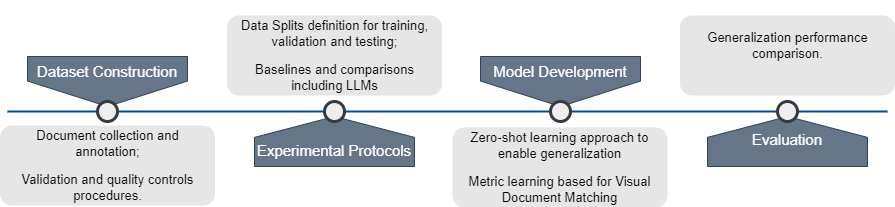
\includegraphics[width=\textwidth, trim={0em 0em 0em 0em},clip]{images/Pipeline Pesquisa 1.png}
% \caption{Overview of the proposed \glsfirst{LA-ZSL} methodology for \glsfirst{VDM}.\label{fig1}}
% \end{figure}  

\section{Dataset Construction}
\label{sec:method_dataset}

% The proposed dataset, \gls{LA-CDIP}, is built as a reorganization of the RVL-CDIP \cite{harley2015rvlcdip} dataset. While RVL-CDIP's classes are divided by their meaning and written content of the documents, the dataset is divided by the visual information and layout. This is illustrated in Figure \ref{img:dataset}, where both groups of documents are classified as the same class under RVL-CDIP, both being forms, but are re-arranged to be different classes under OL-CDIP, as they are visually distinct. 

In the literature, solutions commonly exploit the pre-trained knowledge of \glspl{LLM} for document classification~\cite{sinha_cica_2024,scius-bertrand_zero-shot_2025}. This approach is motivated by the observation that models trained from scratch in \gls{ZSL} settings often fail to adequately separate unseen classes, particularly those classes defined by purpose. Khalifa et al.~\cite{khalifa_contrastive_2023} extensively studied the viability of using contrastive learning~\cite{chopra_learning_2005} to enable zero-shot \gls{DIC}. However, despite the robust design of their method, the observed F1 score of only 69.9\% indicates that \gls{RVL-CDIP} is unsuitable for \gls{ZSL} tasks. Additionally, Larson et al.~\cite{larson_evaluation_2023} highlighted this difficulty by stating that each \gls{RVL-CDIP} class comprises various subclasses. They further argue that this may constrain \gls{ZSL} solutions, as no single reference could specify an entire class without overlaps.

In order to address the setbacks pointed out by Larson et al., we propose the \glsfirst{LA-CDIP} dataset to support zero-shot \gls{DIC} and \gls{VDM}. This dataset focuses on separating documents by their structural pattern, rather than their purpose. Visual cues such as a company logo, the layout of a table, the position of certain text, etc., all contribute to differentiating between distinct document patterns, and different patterns imply different classes. While the \gls{RVL-CDIP} dataset was used as source content, it was re-labeled to align with the problem of differentiating documents, with a particular focus on their visual structure (layout). 

\begin{figure}[htbp]
  \centering
\includegraphics[width=.455\textwidth]{images/class_comparison1.png} \hspace{.04\textwidth}
    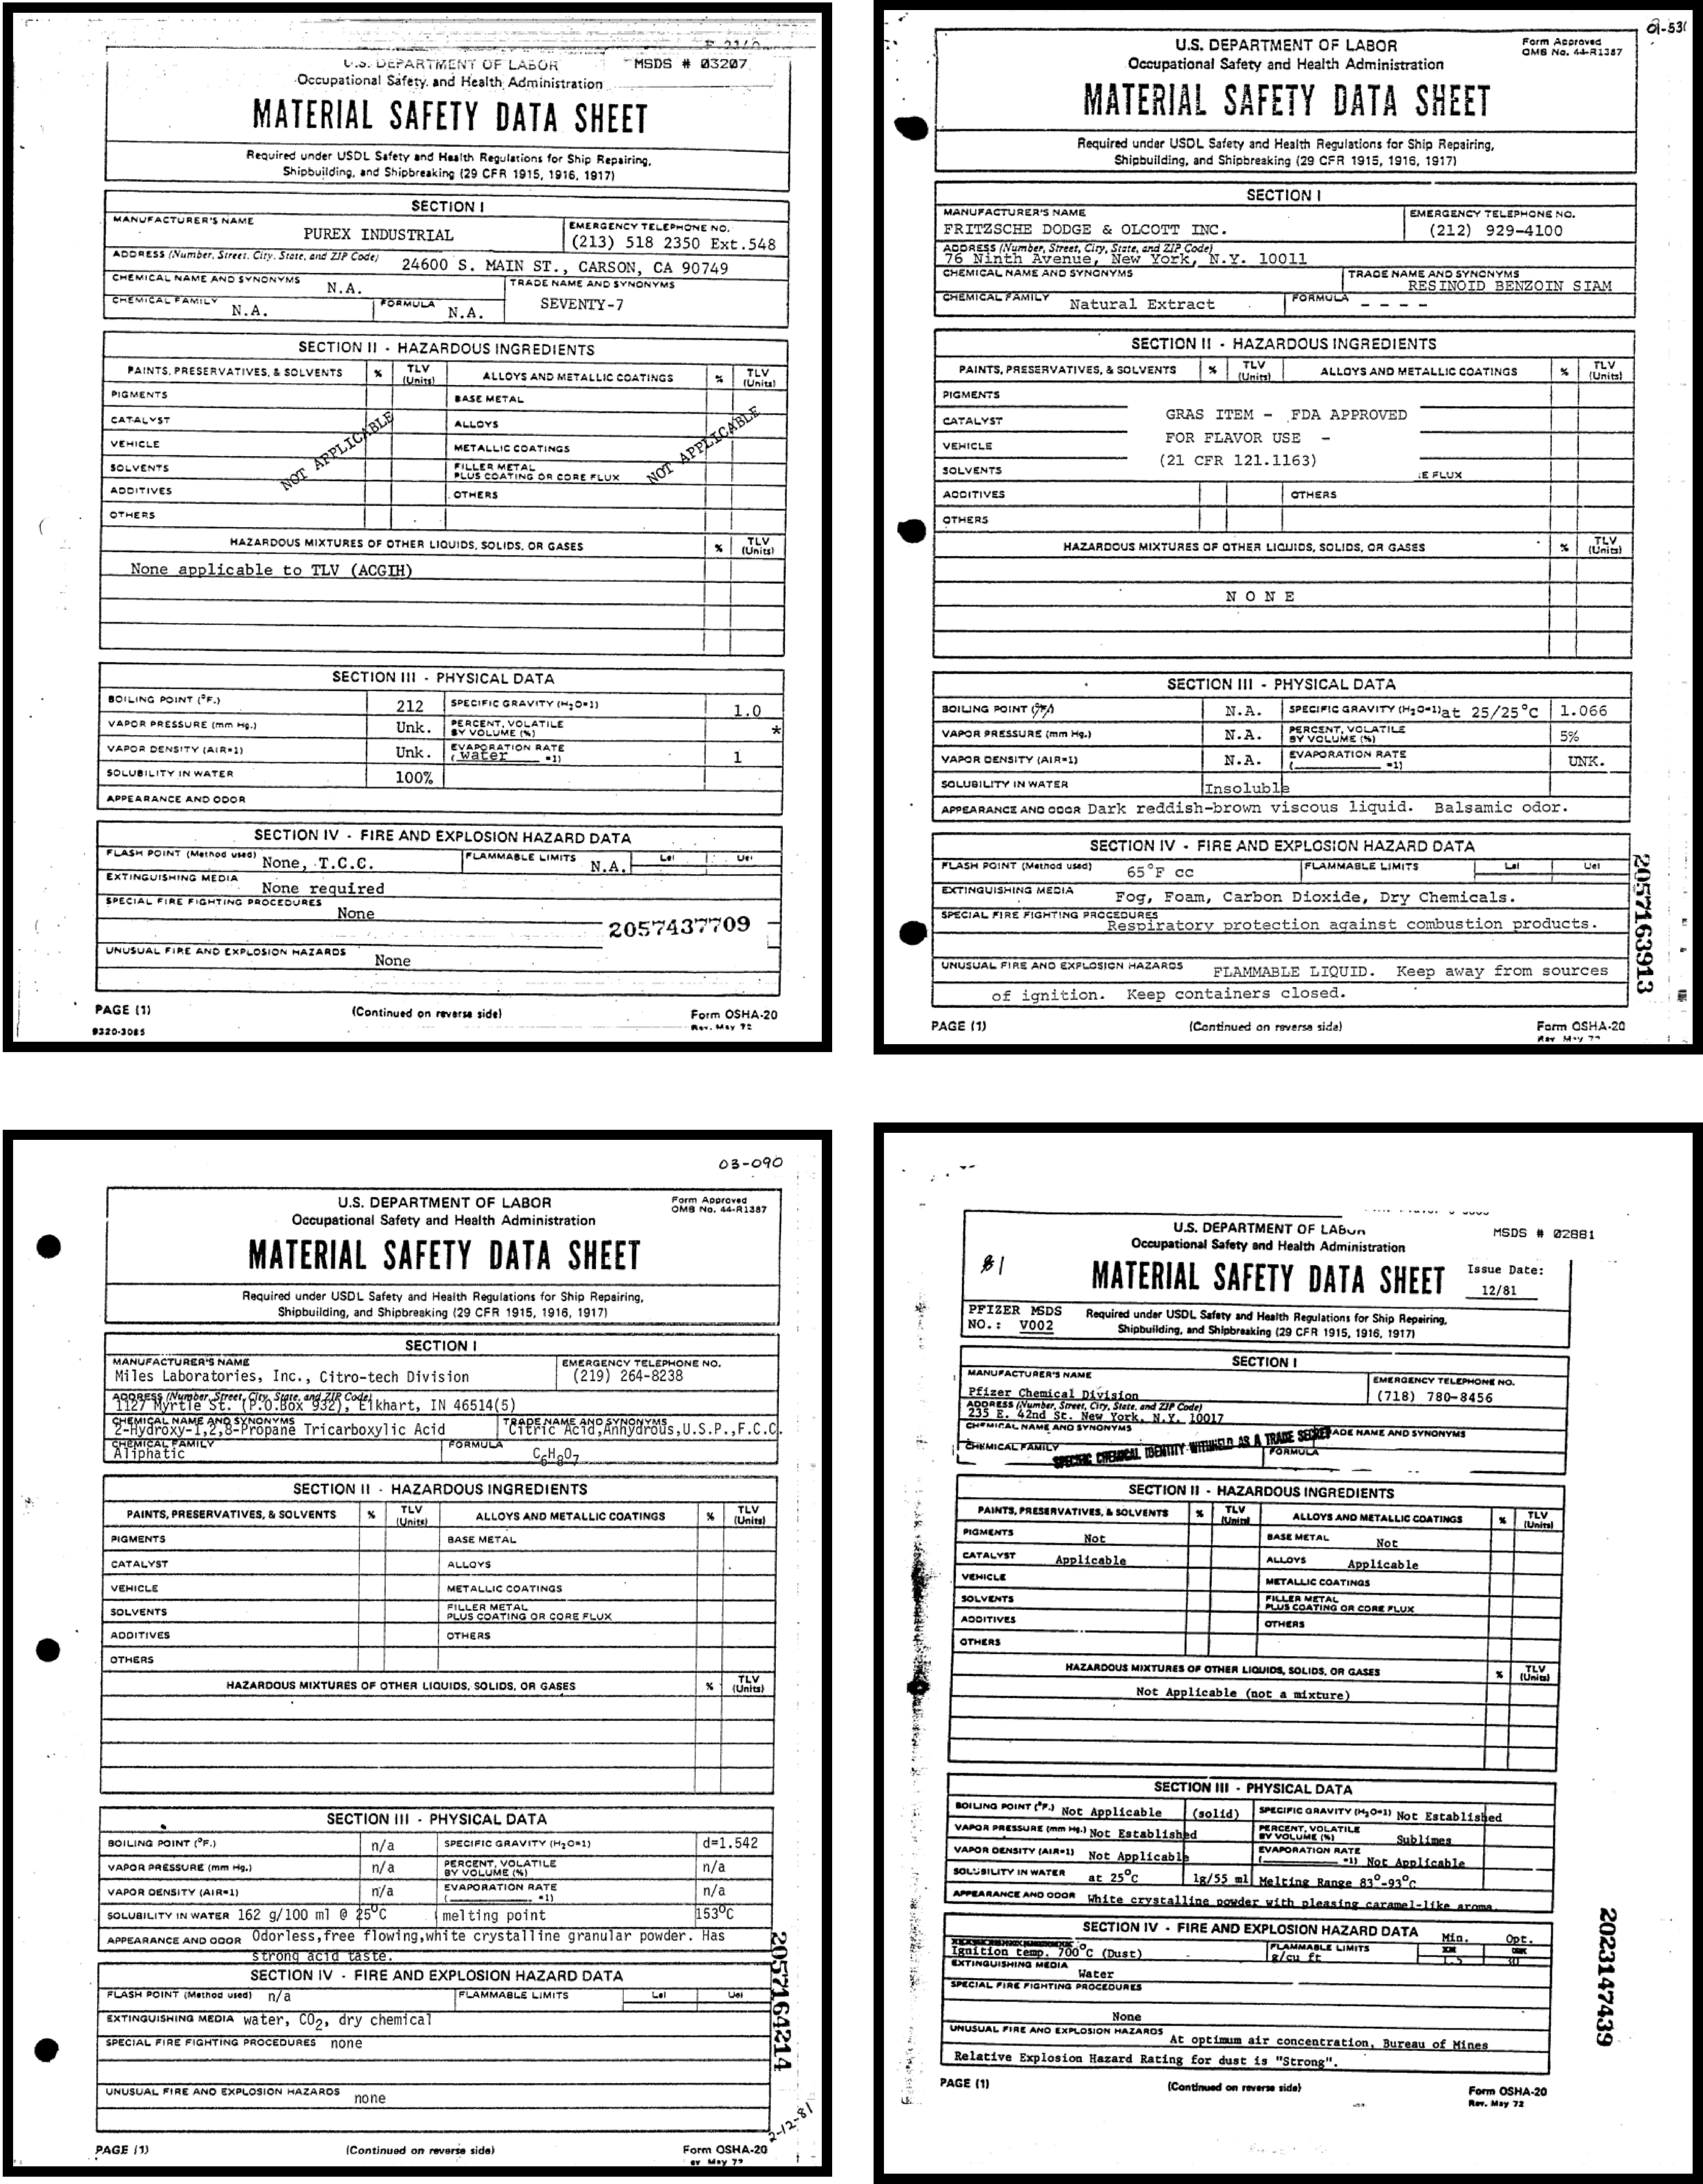
\includegraphics[width=.455\textwidth]{images/class_comparison2.png}

\caption{Examples of two distinct classes under the proposed \gls{LA-CDIP} dataset. Those classes originally belonged to the same class under RVL-CDIP organization.\label{img:dataset}}
\end{figure}   

The construction of the database followed a light active learning framework (see \refCap{sec:active_learning}), following two stages: preliminary clustering, followed by a manual reorganization. The clustering is made with a private metric learning model, trained with a private document dataset, with both the model and the dataset following the same methodology as this thesis. To generate the clusters, the trained model is used to generate a feature vector for every document in the \gls{RVL-CDIP} dataset. Next, the Hierarchical Agglomerative Clustering algorithm, with Ward's\cite{ward_jr_hierarchical_1963} strategy, is employed. This algorithm allows the creation of a dynamic number of clusters, as opposed to a fixed $k$ number of clusters required, for example, by k-Means. This is important due to the \gls{ZSL} nature of the problem, as the resulting dataset needs to achieve layout and class diversity, in other words, achieve a large number of classes. This clustering served the purpose of accelerating the manual labeling process.

Through the manual labeling process, the clustering served exclusively as suggestions, as the clusters themselves were not homogeneous, nor unique, and therefore could not be taken as ground truth. The manual labeling process was separated into two steps: first, given a cluster to analyze, clean the cluster so there is only one document pattern in the cluster. And for the second step, verify if this cluster shares a document pattern with another cluster. If so, merge both clusters into one. To ensure quality of the proposed dataset, a second independent validation of the dataset is conducted, reviewing both intra-class and inter-class consistency and fixing occasional human errors.

\section{Leveraging LLM for Benchmarking Visual Document Matching}
\label{sec:method_benchmark}

A structured prompt that guides \gls{LLM} to compare two document images is used to benchmark \gls{VDM}, evaluating visual similarity. Models were asked to assign a similarity score from 0 to 100, categorized into five levels: Nearly Identical, Highly Similar, Moderately Similar, Weak Similarity, and Completely Different. This evaluation was carried out using Google Colab~\cite{research_google_2024}, where the size of the model and the computational resources were limited. \refFig{fig:document_comparison} illustrates the input-output structure of the document comparison framework. The left and right images represent the document pairs analyzed by \glspl{LLM}, which generate a similarity score and a categorical classification.

\begin{figure}[htbp]
    \centering
    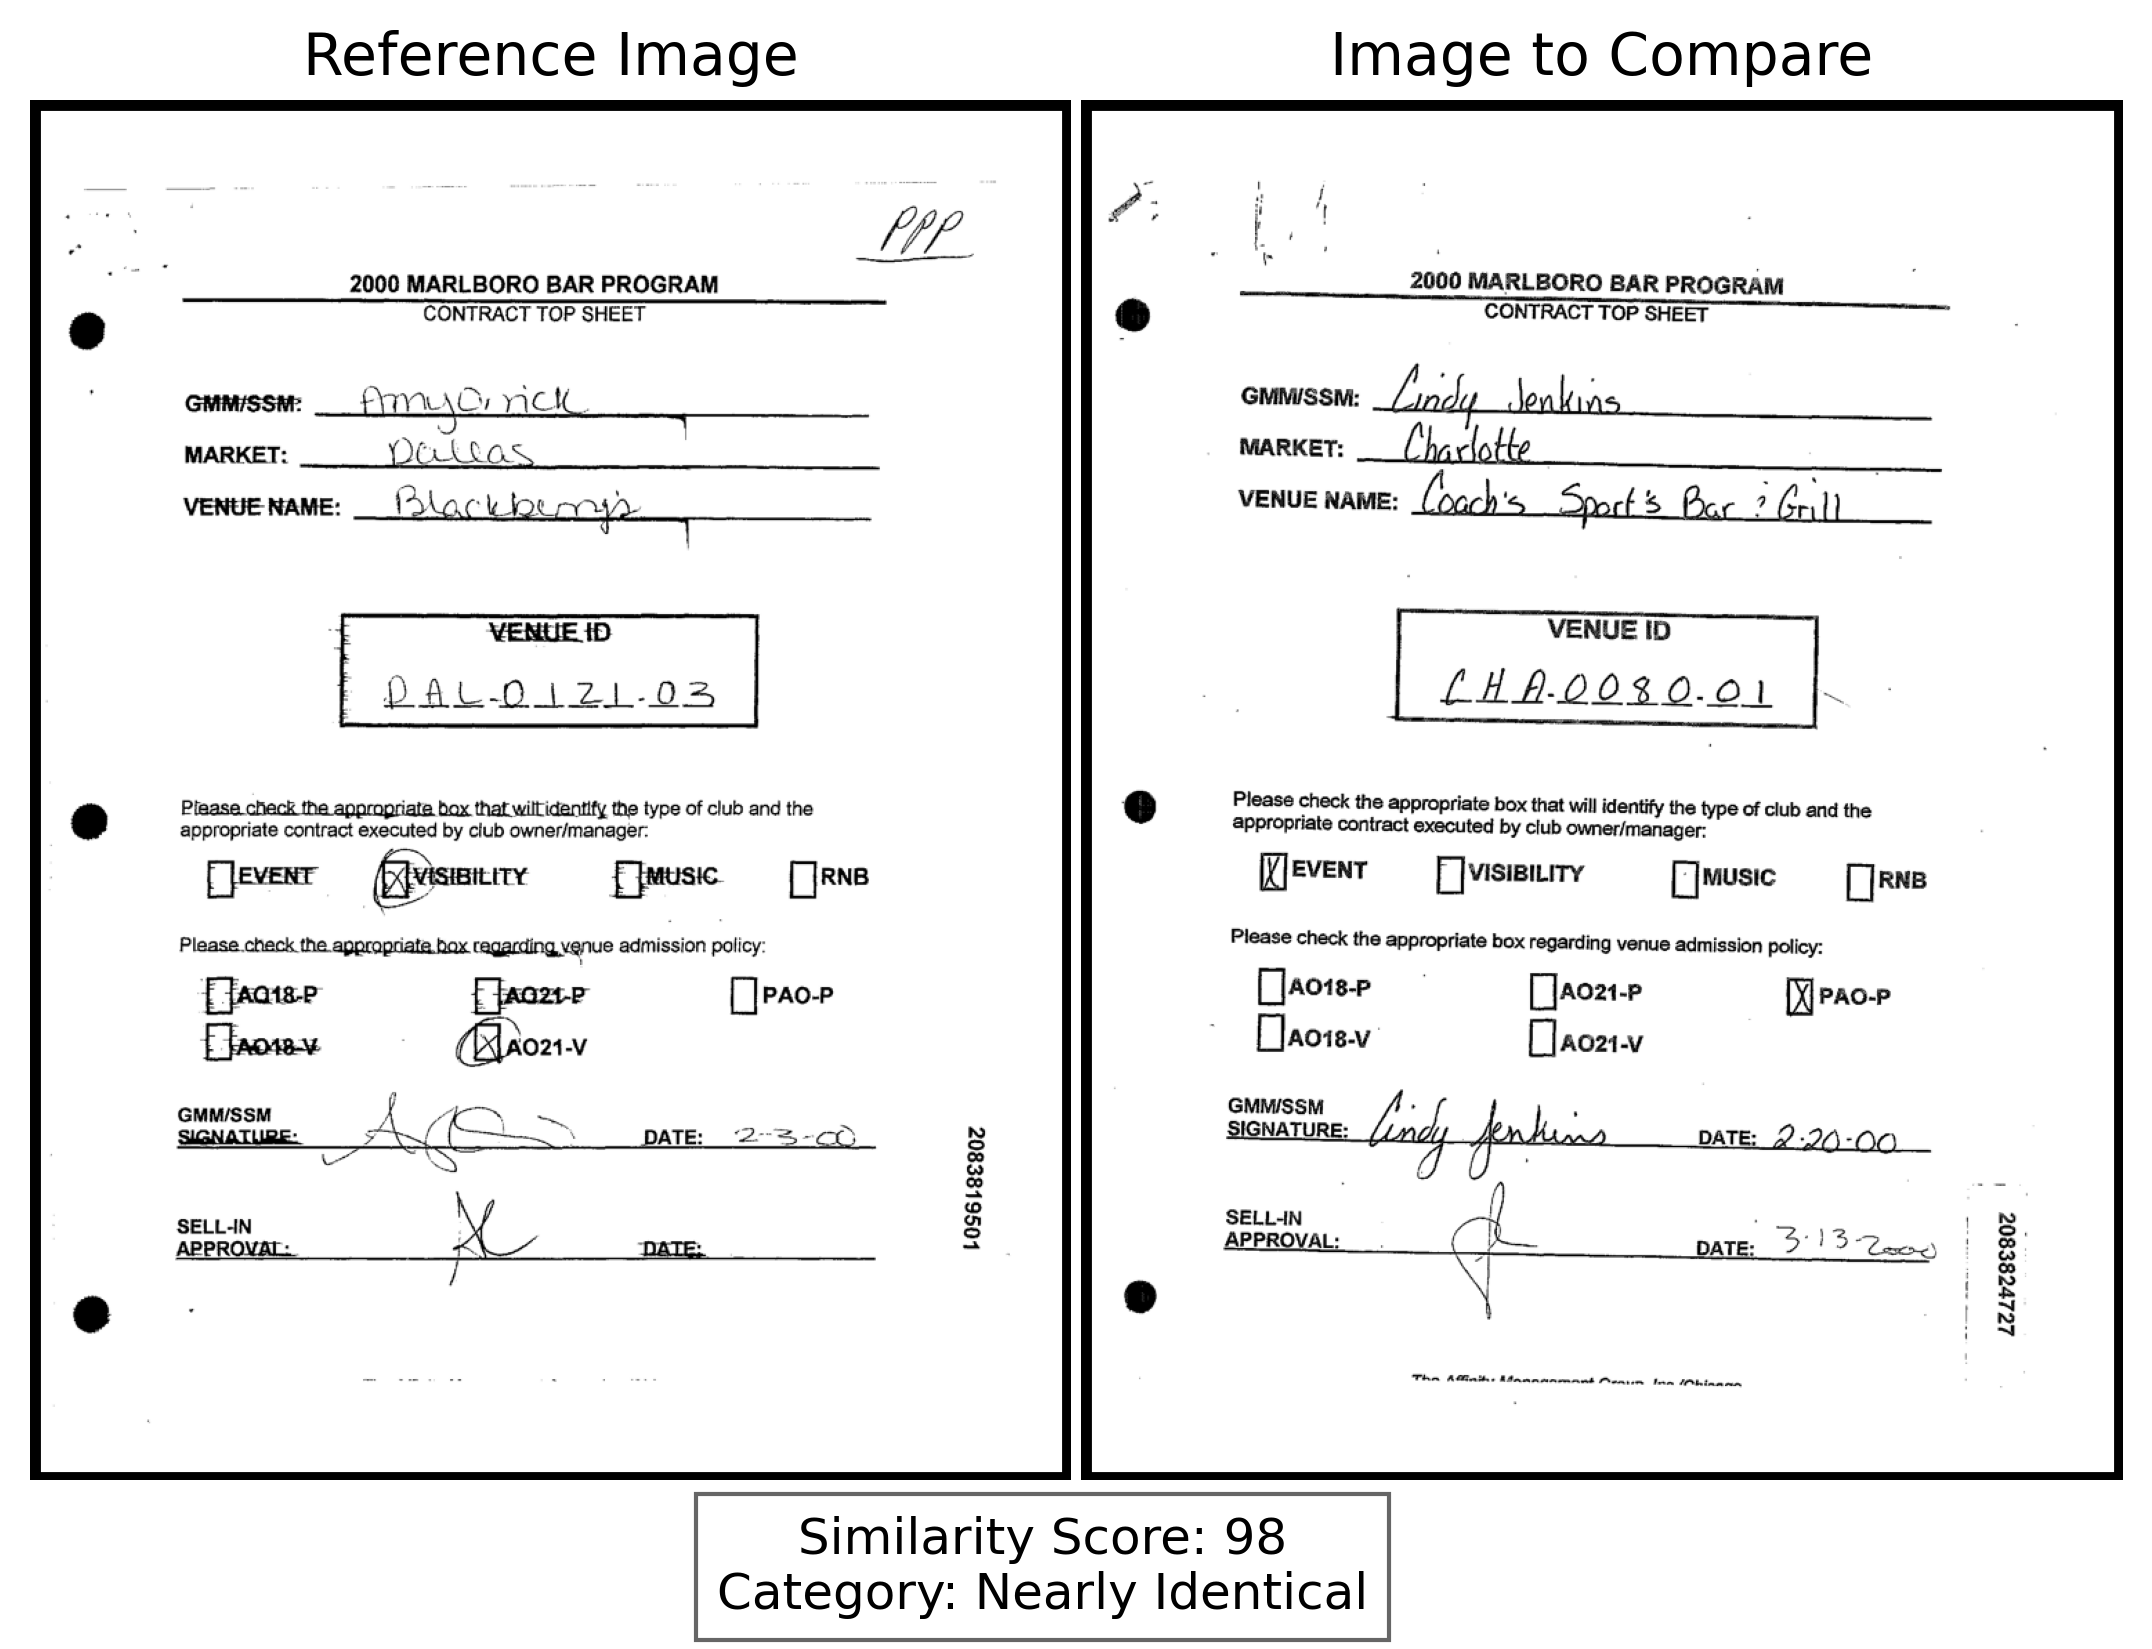
\includegraphics[width=.8\linewidth]{images/similar.png}
    \\[1em]
    \centering
    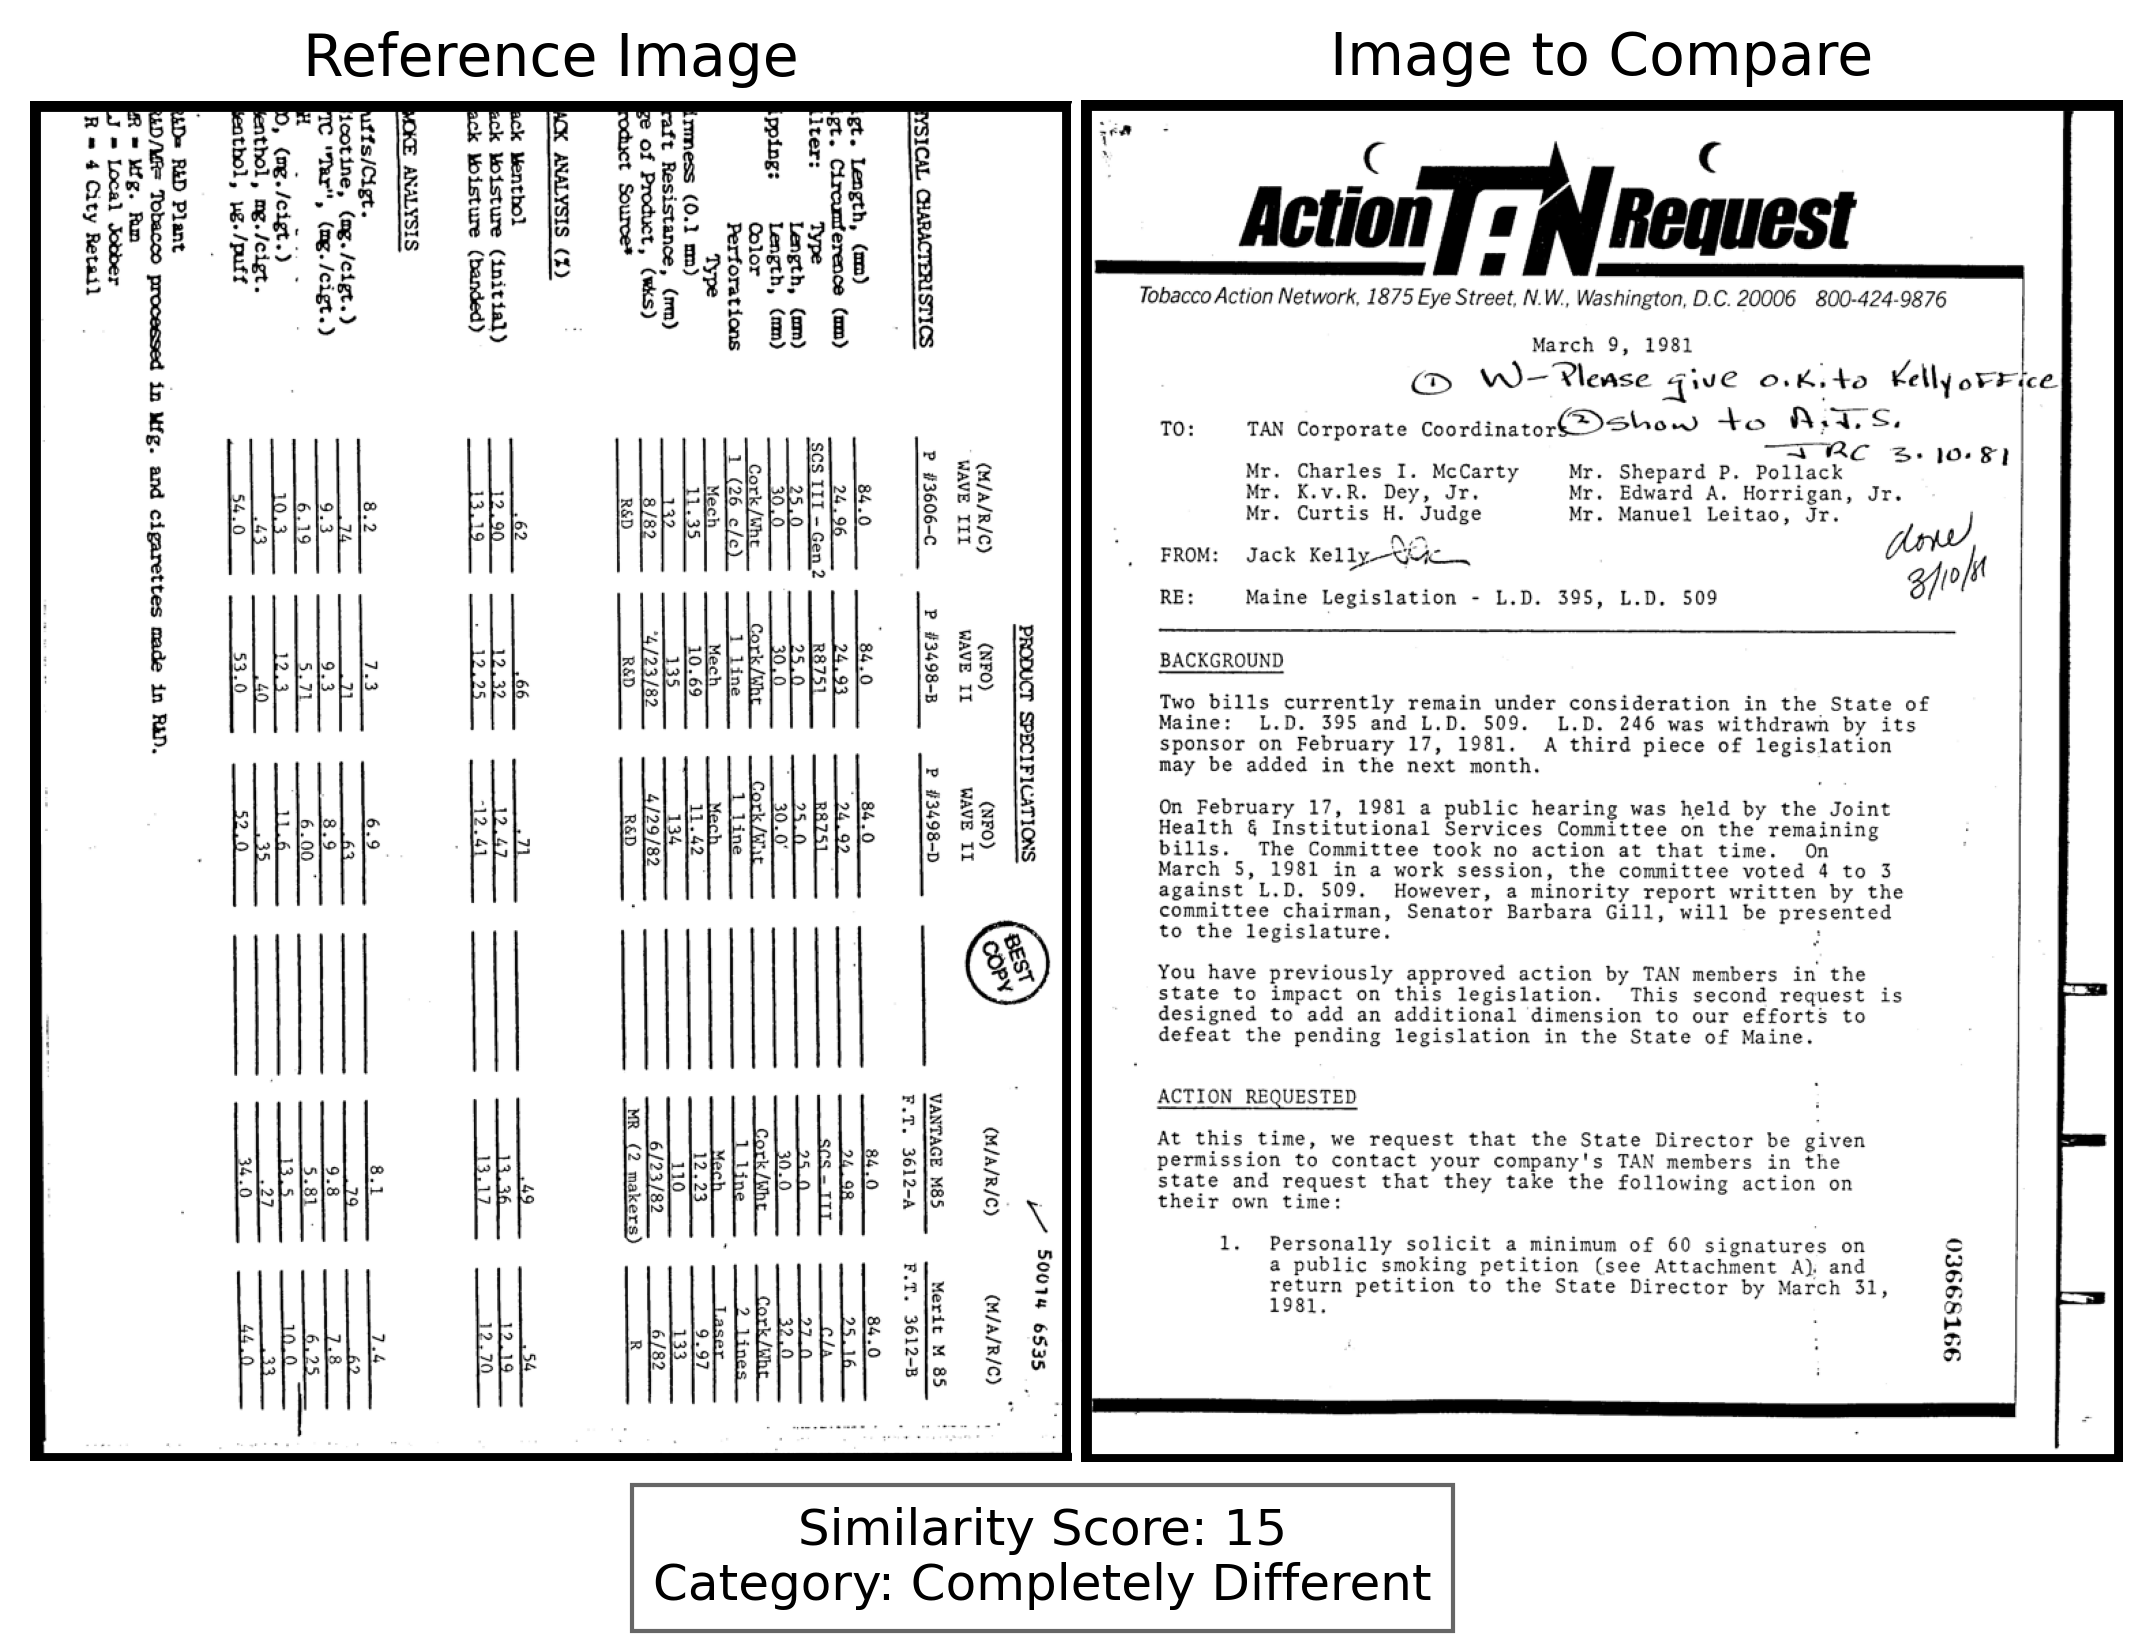
\includegraphics[width=.8\linewidth]{images/different.png}
    \caption{Two sets of comparisons by a LLM model. The first example shows the same layout, and the second, different layouts. The scores range from 0 to 100.}
    \label{fig:document_comparison}
\end{figure}

\section{Visual Document Matching}
\label{sec:method_modeling}

Traditional classification methods, such as entropy learning, lock the generality of the model to the set of classes it has been trained on. Therefore, the use of Zero Shot Learning techniques are essential to be able to classify document layouts that have not been seen on the training set. A wide variety of backbones are used to experiment on the proposed dataset, but they all follow the same metric learning architecture with Siamese Networks.

The dataset is benchmarked by choosing traditional, well established vision Neural Networks as the backbones. They are ResNet~\cite{he_deep_2016}, MobileNetV3~\cite{howard_searching_2019}, EfficientNet~\cite{tan_efficientnet_2019}, VGG~\cite{simonyan_very_2015}, \gls{ViT}~\cite{dosovitskiy_image_2021}. To adapt the architectures to a siamese network, only the last linear layer of each model---the classification layer---is modified into a new linear layer with an arbitrary size $n$, suitable for the problem. In summary, the model learns to draw a representation of an input document in a feature space with $n$ dimensions, such that documents that share the same class are represented clustered together, and documents that have different classes are far apart, as illustrated in \refFig{fig:vector_space_mapping}.

\begin{figure*}[ht!]
    \begin{subfigure}[b]{0.99\textwidth}
        \centering
        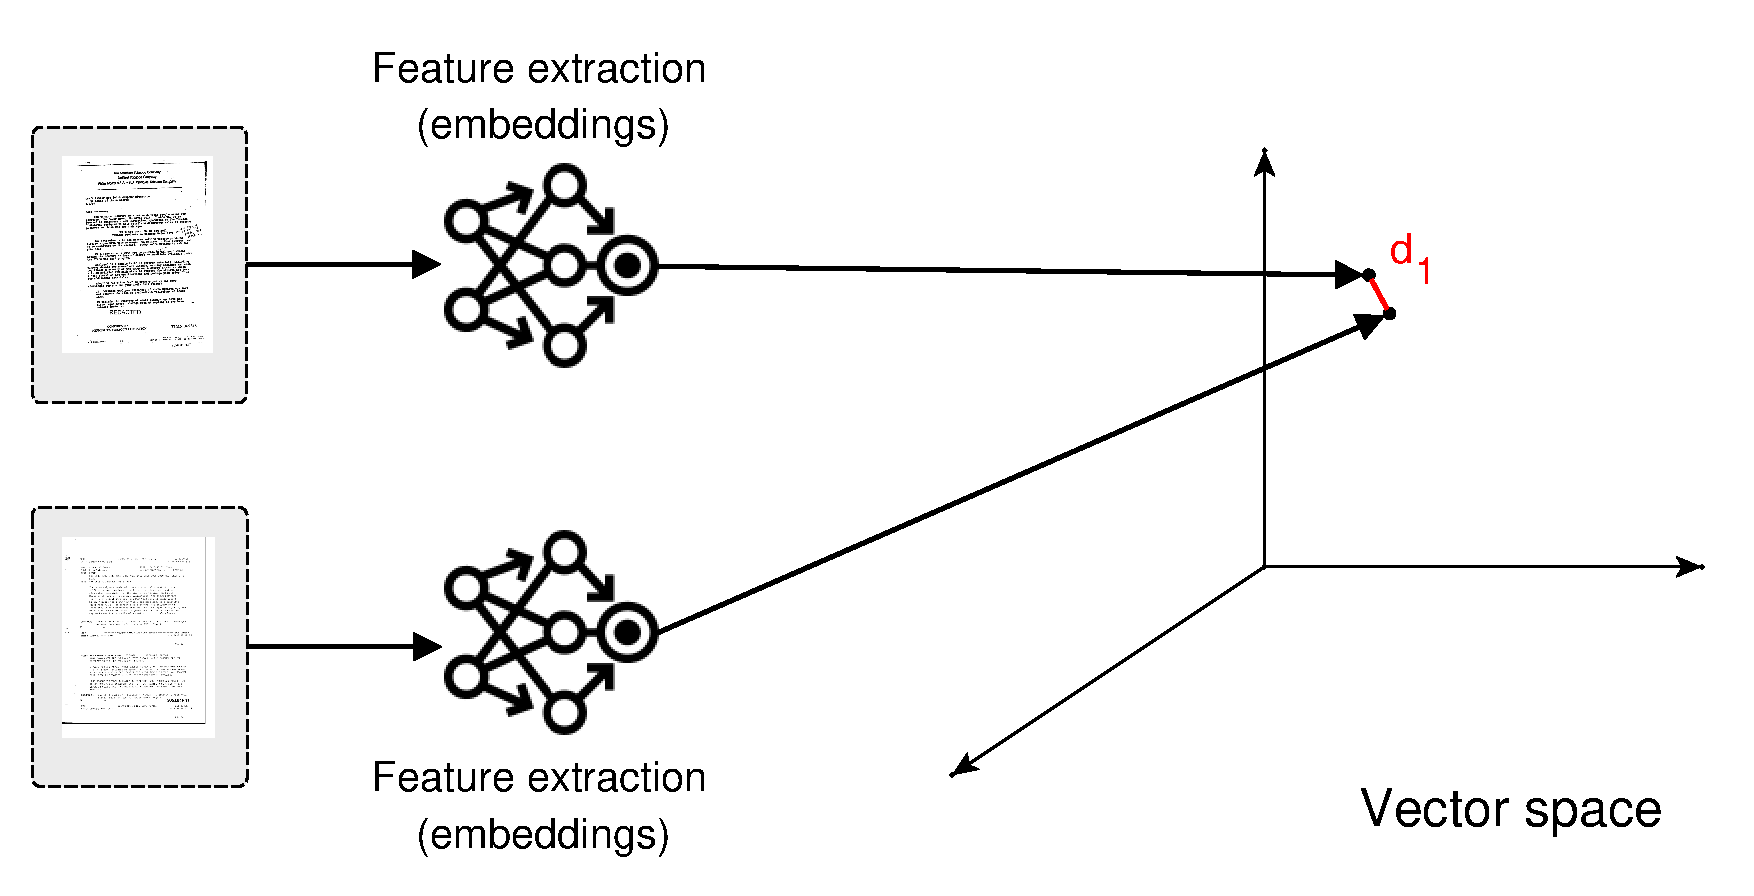
\includegraphics[width=\textwidth, trim=15 0 30 0, clip]{images/vector_space_1.pdf}
        \caption{Similar documents with small distance $d_1$ between them.}
        \label{fig:similar_docs}
    \end{subfigure}
    \vfill
    \begin{subfigure}[b]{0.99\textwidth}
        \centering
        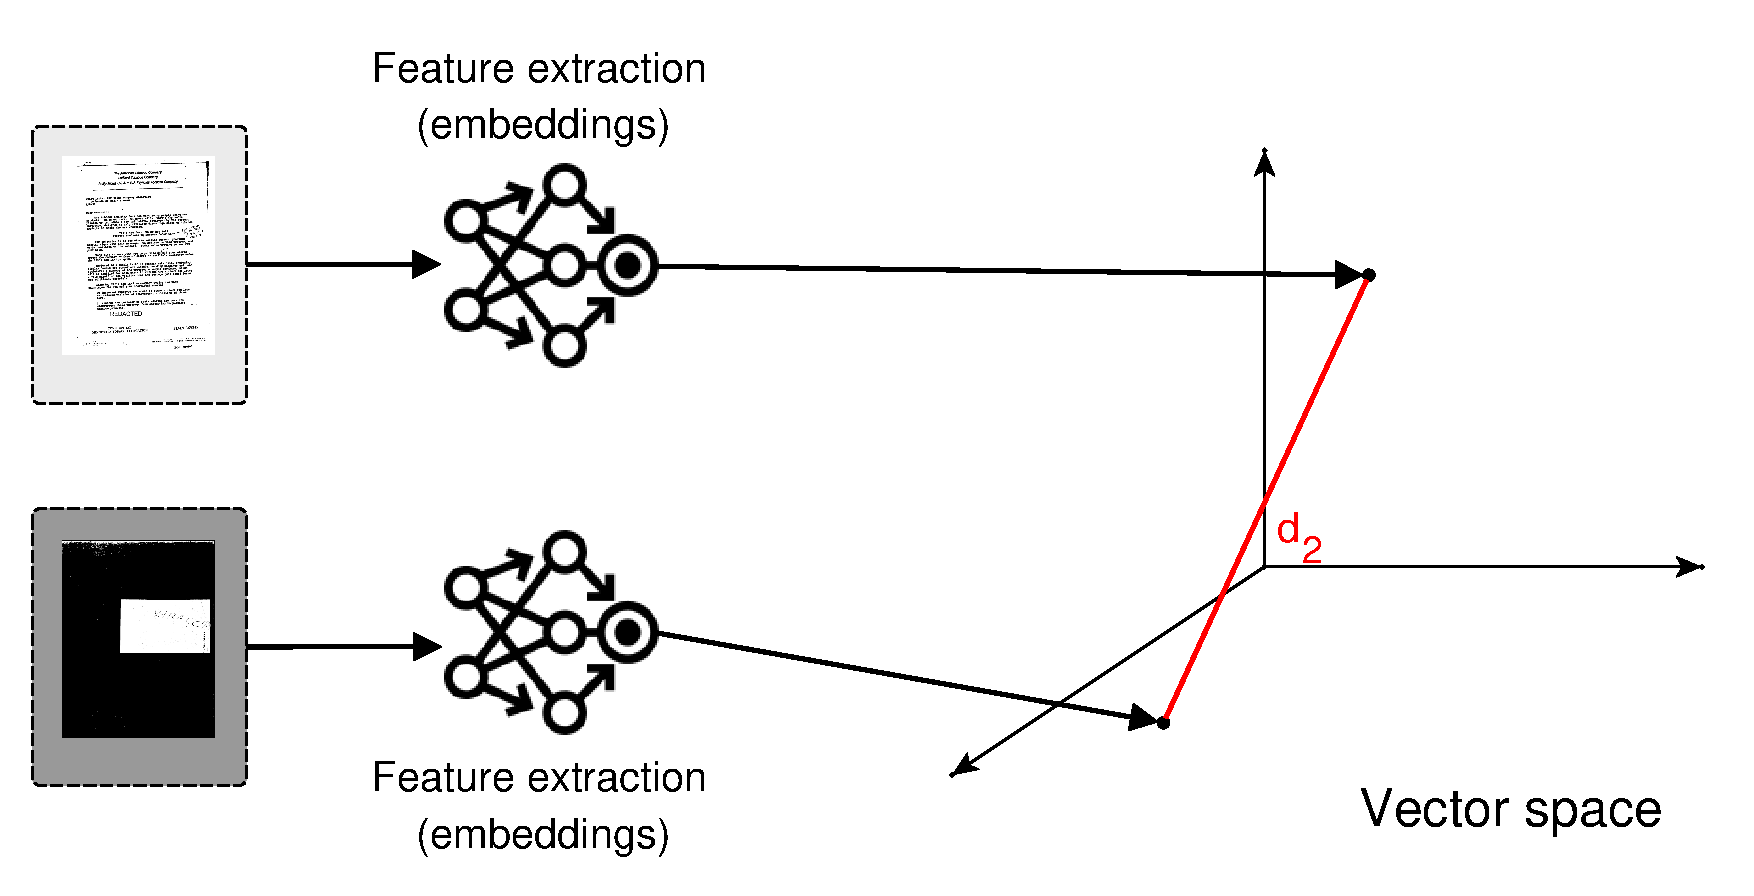
\includegraphics[width=\textwidth, trim=15 0 30 0, clip]{images/vector_space_2.pdf}
        \caption{Dissimilar documents with large distance $d_2$ between them.}
        \label{fig:dissimilar_docs}
    \end{subfigure}
    \caption{Illustration of two documents mapped to the vector space that are similar (a) and dissimilar (b). This document mapping to a vector space is performed by the proposed learned method for similarity analysis. Visually similar documents have a smaller distance in the projected space than dissimilar ones.}
    \label{fig:vector_space_mapping}
\end{figure*}

The trained models are exclusively visual; therefore, their input data is the $(R, G, B)$ document image matrix. First, the input image is resized into a shape compatible with each neural architecture. For most models, this shape is $(224, 224)$ in height and width. EfficientNet is the only architecture that does not follow this rule, as the different model versions increase their input size at the same time they increase the network depth and width. Then, every value of the image matrix is scaled from $0\text{--}255$ to $0\text{--}1$, and normalized with the mean and standard deviation of the current training split. During a training epoch, for each document in the dataset, a random document is chosen to form a pair. Every class has the same odds of being chosen to mitigate overfitting in predominant classes. No data augmentation and no pair mining are used in these experiments. The models are trained with a supervised contrastive learning framework, and use the Contrastive Loss~\cite{chopra_learning_2005} as the loss function.